\documentclass[acmsmall,review,anonymous]{acmart}\settopmatter{printfolios=true,printccs=false,printacmref=false}
\acmJournal{PACMPL}
\acmVolume{1}
\acmNumber{OOPSLA} % CONF = POPL or ICFP or OOPSLA
\acmArticle{1}
\acmYear{2018}
\acmMonth{1}
\acmDOI{} % \acmDOI{10.1145/nnnnnnn.nnnnnnn}
\startPage{1}
\setcopyright{none}
\bibliographystyle{ACM-Reference-Format}
\citestyle{acmauthoryear}   %% For author/year citations
\usepackage{my_style}
\usepackage{listings, wrapfig,xspace}
\usepackage{paralist}

\lstset{language=R}
\definecolor{LightGray}{rgb}{.92,.92,.92}
\definecolor{Gray}{rgb}{.3,.3,.3}
\definecolor{DarkGray}{rgb}{.5,.5,.5}
\lstset{ %
  columns=flexible,
  captionpos=b,
  frame=single,
  framerule=0pt,
  tabsize=2,
  belowskip=0.5em,
  backgroundcolor=\color{LightGray},
  basicstyle=\small\ttfamily,
  emphstyle=,
  keywordstyle=,
  commentstyle=\color{Gray}\em,
  stringstyle=\color{Gray},
  numbers=left,
  showstringspaces=false
}
\lstdefinestyle{R}{ %
  language=R,
  morekeywords={assign, delayedAssign},
  deletekeywords={env, equal, c, runif, trace, args, exp, t, all},
  breaklines=true
}
\lstdefinestyle{Rin}{ %
  style=R,
  breaklines=false
}

\newcommand{\eg}{\emph{e.g.},\xspace}
\newcommand{\ie}{\emph{i.e.},\xspace}
\newcommand{\cf}{\emph{cf.}\xspace}

\newcommand{\PIR}{\textsf{PIR}\xspace}
\newcommand\pirI[1]{\mathtt{#1}}
\renewcommand{\c}[1]{{\lstinline[style=Rin]!#1!}\xspace}
\newcommand{\code}[1]{{\lstinline[style=Rin]!#1!}\xspace}
% Macros for type names from the old paper.
\newcommand{\attr}[2]{\ensuremath{#1_{\mathtt{#2}}}\xspace}
\newcommand{\attrclass}[3]{\ensuremath{#1^{\mathtt{#3}}_{\mathtt{#2}}}\xspace}
\renewcommand{\to}{\ensuremath{\rightarrow}\xspace}
\newcommand{\D}{\ensuremath{\small\vec{\mathtt D}}\xspace} % Double
\newcommand{\I}{\ensuremath{\small\vec{\mathtt I}}\xspace} % Integer
\renewcommand{\C}{\ensuremath{\small\vec{\mathtt C}}\xspace} % Character
\renewcommand{\L}{\ensuremath{\small\vec{\mathtt L}}\xspace} % Logical
\newcommand{\R}{\ensuremath{\small\vec{\mathtt R}}\xspace} % Raw
\newcommand{\X}{\ensuremath{\small\vec{\mathtt X}}\xspace} % Complex
\newcommand{\Y}{\ensuremath{\small\vec{\mathtt Y}}\xspace} % Symbol
\newcommand{\sY}{\ensuremath{\small{\mathtt Y}}\xspace} % Symbol
\newcommand{\sS}{\ensuremath{\small{\mathtt S}}\xspace} % S4
\newcommand{\sF}{\ensuremath{\small{\mathtt F}}\xspace} % Closure
\newcommand{\sE}{\ensuremath{\small{\mathtt E}}\xspace} % Env
\renewcommand{\R}{\ensuremath{\small\vec{\mathtt R}}\xspace} % Raw
\newcommand{\sN}{\ensuremath{\small{\mathtt N}}\xspace}     % Null
%\renewcommand{\l}{\ensuremath{\small L<?>}\xspace}     % List
\renewcommand{\l}{\ensuremath{\small\underline{\mathtt ?}}\xspace}     % List
\newcommand{\sD}{\ensuremath{\small{\mathtt D}}\xspace} % Double
\newcommand{\sI}{\ensuremath{\small{\mathtt I}}\xspace} % Integer
\newcommand{\sC}{\ensuremath{\small{\mathtt C}}\xspace} % Character
\newcommand{\sL}{\ensuremath{\small{\mathtt L}}\xspace} % Logical
\newcommand{\sX}{\ensuremath{\small{\mathtt X}}\xspace} % Complex
\newcommand{\sR}{\ensuremath{\small{\mathtt R}}\xspace} % Raw
\newcommand{\ANY}{\ensuremath{\small{\mathtt ?}}\xspace}     % Any
\newcommand{\lT}[1]{\ensuremath{\small\underline{\mathtt{#1}}}\xspace}     % list<T>
\newcommand{\M}[1]{\ensuremath{\attr{\vec{\tt #1}}{mat}}\xspace}     % matrix
\newcommand{\df}{\ensuremath{\attr{\l}{df}}\xspace}     % data.frame

\newcommand{\contractr}{\emph{contractr}\xspace} % contractr
\newcommand{\roxygen}{\emph{roxygen2}\xspace} % roxygen
\newcommand{\typetracer}{\emph{typetracer}\xspace} % typetracer
\newcommand{\rdt}{\emph{R-dyntrace}\xspace}
\newcommand{\covr}{\emph{covr}\xspace}




\begin{document}
\title{Extracting Function Signature from R Program Traces}

\begin{abstract}
  This paper documents the first steps towards retrofitting a type system
  onto the R programming language. We introduce an extension of R with
  function signatures. To evaluate the fit of our design to the language, we
  start by automatically extracting the signatures for 500 widely used
  packages. In a second step we use the reverse dependencies of these
  packages to validate that these signatures are accurate.
\end{abstract}
\maketitle


\section{Introduction}

How does one retrofit a type system to an existing language? Three succesful
models are Hack, Typed Racket and TypeScript. 


The story that we're aiming for: Designing type systems for established
languages can be a challenging.  We aim to approach this problem by
essentially reverse-engineering a type system from a corpora analysis of a
representative subset of R code.  We present a simple type system that
captures the vast majority of usage of R --- it is lightweight, and
\AT{should provide enough information to be useful to a compiler}.

To evaluate our type system, we present a type-checker that is aware of R's
promise semantics.  In R, function arguments are wrapped in promises such
that they are not evaluated until they are needed.  Our tool deals with
these promises by inserting a check which fires only when the promise is
forced, at which point the value is checked for compliance with the type.


%
%
%
\section{Background}

In this section, we will introduce the R programming language, as well as discuss the dynamic analysis framework we used as part of our initial analysis.

%
%
%
%
\subsection{The R Programming Language}
\label{sec:R}

Over the last decade, the R Project has become a key tool for implementing
sophisticated data analysis algorithms in fields ranging from Computational
Biology~\cite{R05} to Political Science~\cite{R:Keele:2008}. At the heart of
the R project is a \emph{vectorized, dynamic, lazy, functional,
  object-oriented} programming language with a rather unusual combination of
features~\cite{ecoop12} designed to ease learning by non-programmer and
enable rapid development of new statistical methods.  The language, commonly
referred to as R was designed in 1993 by Ross Ihaka and Robert
Gentleman~\cite{R96} as a successor to S~\cite{S88}.  First released in
1995, under a GNU license, R rapidly became the lingua franca for
statistical data analysis. Today, there are over 13,000 R packages available
from repositories such as CRAN and Bioconductor.  With 55 R user groups
world-wide, Smith~\cite{eco11} estimates that there are over 2 million
end-users.

As an introduction to R, consider the code snippet in Fig.~\ref{sample} from
a top-level interaction where the user defines a function \code{normSum}
that accepts vectors of integers, logicals, doubles and complex values and
normalizes the vector with respect to its sum and rounds the results. The
function definition does not require type annotations, and all operations
transparently work on vectors of any length and different types.

\begin{figure}[!hb]{\small
\begin{lstlisting}
> normSum <- function( m )  round( m / sum(m), 2)
> normSum(c(1L,3L,6L))
[1] 0.1 0.3 0.6
> normSum(c(1.1,3.3,6.6))
[1] 0.1 0.3 0.6
> normSum(c(1.6,3.3,6.1))
[1] 0.15 0.30 0.55
> normSum(complex(r=rnorm(3),i=rnorm(3)))
[1] 0.49+0.21i 0.30-0.18i 0.22-0.03i
\end{lstlisting}}
\caption{Sample R code}\label{sample}
\end{figure}

In R, function can be called with named parameters, R support variable
argument lists, and arguments can have default values. Putting all of these
together consider the following declaration:

\begin{lstlisting}
f <- function(x, ..., y=3) x + y
\end{lstlisting}

\noindent
Function \k{f} can be called with a single argument \code{f(3)}, with named
argument \code{f(y=4,x=2)} and with a variable number of arguments,
\code{f(1,2,3,4,y=5)}, all of these calls will return \code{6}.

R has a number of features that are not crucial to the present
discussion. We will mention some of them here for completeness.  In R, data
structures are reference counted and have copy-on-write semantics, thus the
assignment \code{x[12]<-3} results in an update to a copy of \code{x} unless
the reference count on that object is 1.  This semantics gives R a
functional flavor while allowing updating in place within loops (the first
update copies, subsequent updates are performed on the copy). Arguments to
functions are evaluated only when needed, they are bundled in so-called
promises which package the original expression (as an abstract syntax tree, or AST), its environment
as well as the result of evaluating the expression. Promises can be
leveraged for meta-programming as it is possible to retrieve the text of a
promise and evaluate it in a different environment.


\subsubsection{Types of Data}
\label{subsubsec:backgroundtypes}

Before attempting to define a type system for R, we should understand the
different kinds of values that programs operate on.  As we will see
different notions of type may emerge depending on how granular we want to
be.

\renewcommand{\k}[1]{{\tt #1}\xspace}

R has one builtin notion of type that can be queried by the \k{typeof}
function. Over the years, programmers have found the need for a richer type
structure and have added {\it attributes}. The best way to think of attributes is
as an optional map from name to values that can be attached to any object.
Attributes are used to encode various type structures. They can be queried
with functions such as \k{attributes} and \k{class}.

\begin{wrapfigure}{r}{6.1cm}
\footnotesize\begin{tabular}{l|c|l@{}}\hline
\multicolumn{3}{l}{\bf Vectorized data types:}  \\\hline
\k{logical}   & \L & vector of boolean values\\
\k{integer}   & \I & vector of 32 bit integer values\\
\k{double}    & \D & vector of 64 bit floating points\\
\k{complex}   & \X & vector of complex values\\
\k{character} & \C & vector of strings values\\
\k{raw}       & \R & vector of bytes\\
\k{list}      & \l & vector of values of any type\\\hline
\multicolumn{3}{l}{\bf Scalar data types:}\\\hline
\k{NULL}      & \sN &  singleton null value\\
\k{S4}        & \sS &  instance of a S4 class \\
\k{closure}   & \sF & a function with its environment\\
\k{environment}&\sE &  a mapping from symbol to value \\\hline
\multicolumn{3}{l}{\bf Implementation data types:}\\\hline
\multicolumn{3}{l}{\k{special},
\k{builtin},
\k{symbol} (\sY),
\k{pairlist},
\k{promise}}\\
\multicolumn{3}{l}{
\k{language},
\k{char},
\k{...},
\k{any},
\k{expression},
}\\
\multicolumn{3}{l}{
\k{externalprt},
\k{bytecode},
\k{weakref}}\\\hline
\end{tabular}\caption{Builtin Types}\label{types}\end{wrapfigure}

Figure~\ref{types} lists all of the builtin types that are provided by the
language. They are the possible return values of \k{typeof}. There is no
intrinsic notion of subtyping in R. But, in many context a \k{logical} will
convert to \k{integer}, and an \k{integer} will convert to \k{double}.  Some
off conversion can occur in corner cases, such as \k{1<"2"} holds and
\k{c(1,2)[1.6]} returns the first element of the vector, as the double is
converted to an integer. R does not distinguish between scalars and vectors
(they are all vectors), so \code{typeof(5) ==} \code{typeof(c(5)) ==
  typeof(c(5,5))} \code{ == "double"}. Finally all vectorized data types have a
distinguished missing value denoted by \code{NA}. The default type of
\code{NA} is \k{logical}. We can see that \code{typeof(NA)=="logical"}, but
NA inhabits every type: \code{typeof(c(1,NA)[2])=="double"}.

With one exception all vectorized data types are monomorphic, the exception
is the \k{list} type which can hold values of any other type including
\k{list}. For all monomorphic data types, attempting to store a value of a
different type will cause a conversion. Either the value is converted to the
type of vector, or the vector is converted to the type of the value.

Scalar data types include the distinguished \k{NULL} value, which is also of
type \k{NULL}, instance of classes written using the S4 object system,
closures and environments.  The implementation of R has a number of other
types that are mostly not used by user code, they are listed in
Figure~\ref{types} for reference.

The addition of attributes lets programmers extend the set of types by
tagging data with user-defined attributes. For example, one could define a
vector of four values, \code{x<-c(1,2,3,4)} and then attach the attribute
\k{dim} with a pair of numbers as value: \code{attr(x,"dim")<-c(2,2)}.  From
that point, arithmetic functions will treat \k{x} as a 2x2 matrix. Another
attribute that can be set is the \k{class}.  This attribute can be bound to
a list of class names. For instance, \code{class(x)<-"human"}, set the class
of \k{x} to be \k{human}.  Attributes are thus used for object-oriented
programming. The S3 object system support single dispatch on the class of
the first argument of a function, whereas the S4 object system allows
multiple dispatch (on all arguments). Some of the most widely used data
type, such as data frames, leverage attributes. A data frame, for instance,
is a list of vectors with a class and a column name attribute.

\paragraph{Summary.} The most common values in R computations are vectorized
types. R programs do not have a way to constrain values to be scalar.
\k{NULL} is sometimes used to represent the case when no value is
available. \k{NA} is used within vector to represent missing observations.
Attributes can decorate values and are used as building blocks for
object-oriented programming. A potential type system for R could focus only
on the builtin types, if one wanted to strive for simplicity, or it could
try to capture attributes at the risk of increased complexity.

%
%
%
%
\subsection{R-dyntrace}
\label{sec:r-dyntrace}

\AT{Leaving this one for Aviral.}

R-dyntrace is an efficient dynamic analysis framework for R.

\subsection{contractr}
\label{sec:contractr}

\AT{I think we should move this to the Methodology section, which we should maybe rename to implementation. Thoughts?}

\contractr is an R package that implements our type system for the R
package ecosystem. It adds contracts to package functions for type-checking
arguments and results on function calls. On contract failure, it reports a type
mismatch warning with the package name, function name, argument name, argument
position, expected type signature, actual type signature of the value observed,
and a stack trace for the called function. \contractr works by modifying
function definition to insert a call to the type-checking function. When the
modified function is called, the type-checking function is invoked on the
modified function's arguments and return value.

\contractr is implemented in 434 R LOC and 2358 C++ LOC. The core
implementation is in C++ to keep the runtime overhead low. It been designed and
tested with GNU R-3.5.0 but it also works with recent versions of R. It has been
hardened with a battery of 400 test cases. We have used it extensively during
the course of this work; firstly, for sanity checking of XXX type signatures
generated for the XXX packages during the development phase, and secondly, for
assessing the quality of these type signatures on XXX packages during the
evaluation phase.

%
%
\subsubsection{Type Declarations}
Type declarations can be made available to \contractr in three ways: as
part of its internal database of types (which already has type signatures for
our corpus of 500 packages), as part of a designated \emph{TYPEDECLARATION} file
supplied by the package author and installed along with the package, or through
a user-level API function insert\_contract that lets the user insert contract to
a custom function with the type declaration provided as a string argument.

%
%
\subsubsection{Challenges}
Retrofitting a robust and efficient type-system as an external package in R has
been a significant undertaking. We had to contend with the complex design
choices of R to make it work without surprises for the end-users. We describe
two key challenges that we faced in the development of \contractr.
\begin{itemize}
\item Firstly, we faced the problem of type-checking arguments in a
  non-strict language while retaining the non-strict semantics. When a
  function is called in R, parameters are bound to unevaluated code thunks
  called promises~\cite{oopsla19}, instead of values which can be
  immediately type-checked. Naively forcing promises at function call to
  obtain a value for type-checking would violate the language semantics,
  leading to incorrect results. To preserve the original semantics,
  \contractr modifies the promise by wrapping the unevaluated promise
  expression in a call to its type-checker along with the context necessary
  to associate the promise to the function and its parameter (for failure
  messages). The contract checking happens when the promise is evaluated,
  either inside the function or many calls deep.  This works, but with one
  wrinkle. GNU R has a bytecode compiler that can sometimes optimize away
  promises; in those cases, \contractr receives values that can be
  immediately type-checked. Non-strict semantics dictate that any
  computation related to the argument should happen on the first use of the
  argument. So type-checking at this point and issuing an error message
  would violate the non-strict semantics; if this argument is never used, it
  would be incorrect to type-check it at the beginning of call. To make this
  work, \contractr mutates the function parameter binding to a promise that
  wraps the argument value in a call to the type-checker, as in the previous
  case.
\item Secondly, we faced the problem of type-checking function return
  value. In R, the result of a function call is the result of evaluating the
  last expression in the function body; so an explicit return call is absent
  from most function definitions. Thus, there could be many potential
  sub-expressions in the function body which need to be type-checked against
  the return type. To address this, \contractr registers the type-checker to
  be called on the return value through a function exit hook. This hook is
  executed in the function call's environment after it has executed. While
  this works, we have to contend with yet another wrinkle, R interpreter can
  perform longjumps in its C implementation, which causes active R function
  calls on the stack to be discarded. When they are discarded, their exit
  hooks are called, which in this case calls the registered
  type-checker. But, these functions are in the middle of an active
  computation, so they don't have a return value to type-check. \contractr
  deals with this problem by allocating a unique sentinel object which
  serves as the return value for calls that are discarded. The function call
  exit hook does not call the type-checker if this unique value happens to
  be the return value of the call.
\end{itemize}
%
%
\subsubsection{Usability}
With \contractr, we aim to provide a hassle-free path to the R developers
for adding types to untyped package code. Hence, we have paid a lot of
attention towards usability in its design. We discuss three such usability
features.
\begin{itemize}

\item \contractr enables automatic type-checking on importing without any
  user intervention. Just running \code{library(contractr)} R code is enough
  to insert contracts, both, in packages pre-loaded in the user's workspace,
  and, in packages that will be loaded eventually. To achieve this
  automation, \contractr relies heavily on R's reflective and dynamic
  capabilities. On loading, \contractr scans all the pre-loaded packages in
  the user's workspace and inserts contracts in functions for which type
  signatures are available. For all other packages installed on user's
  machine but not yet loaded in the workspace, \contractr sets up package
  load hooks which are executed by R when those packages are loaded. The
  hook registered by \contractr insert contracts to those package's
  functions. Thus, developers and users do not have to call the \contractr
  API to enable type-checking for packages at any point of their programming
  workflow. Furthermore, \contractr automatically removes contracts from all
  the package functions and restores them to their original state when it is
  unloaded, an operation that is rarely performed, but useful in interactive
  settings.

\item \contractr enables package authors to supply type declarations for
  their package without requiring package code modifications. Type
  declarations can be written alongside a \code{@type} section inside
  \roxygen function comment blocks. \roxygen is an R package that enables
  authors to add documentation to R functions in the form of organized
  plaintext sections which are automatically exported to R's latex style
  custom documentation format.  \roxygen is a widely adopted package, used
  by over XXX R packages in CRAN. It provides an extension API for adding
  custom documentation tag sections in comment blocks. The sections are
  processed by \roxygen before package build step and a registered method
  for each custom tag section is invoked with the section data and
  documented object. \contractr uses this mechanism to register a hook for a
  custom \code{@type} tag. This hook parses the type declarations from the
  \code{@type} sections, extracts the function name from the documented
  function definition, and stores them in a TYPEDECLARATION file inside the
  package folder. This files is copied verbatim on package installation and
  picked up \contractr when the package is loaded. Here is an example of how
  a roxygen code block looks like with our type declaration:

  This feature enables a function and its type signature to coexist next to each
  other, where they are more likely to remain synchronized. Furthermore, the
  \contractr hook can also add the function's type declaration to its
  documentation, which seamlessly integrate our type system with the existing R
  tooling.
  
\item \contractr provides a very expressive API to the users, covering a
  variety of uses cases. During interactive development, developers can
  explicitly insert contracts by supplying the type declaration as a string
  argument to the \code{insert\_contract} API function. Conversely,
  contracts can be removed by calling the \code{remove\_contract} API on
  functions. Contracts can be selectively enabled or disabled for code
  blocks by wrapping them in calls to \code{ignore\_contracts} and
  \code{capture\_contracts} functions. This enables selective type-checking
  of code section during the development phase.  Furthermore, these
  functions return a data frame that contains all the information about
  failed and successful contract assertions in the wrapped code blocks. This
  is useful for post-hoc investigation. Multiple type-checking failures can
  introduce a lot of noise in the program output. To alleviate this problem,
  \code{contractr.severity} option can be set to \code{'silence'}.  This
  suppresses failure messages but \contractr still performs type-checking
  whose results can be explicitly obtained as a data frame from the
  \code{get\_contracts} API function. R suppresses printing of warnings on
  the terminal when a function issues too many warnings. This can hide
  type-checking failure messages. Setting \code{contractr.severity} flag to
  \code{'error'} turns the type-checking failure warnings to errors, which
  halts the program at the point of contract failure.

\end{itemize}

While \contractr's primary logic has been implemented in C++, we have not
observed a single segfault during our use of the package, either during the
development and sanity-checking phase, or during the evaluation phase.
We conclude the discussion of \contractr by drawing reader's attention to the
engineering effort it takes to package experimental ideas in the form of stable
and easy-to-use tools. R has an eclectic mix of features and design oddities
that make this even harder. 

%
%
%
%
\section{Project Corpus}\label{sec:corpus}

For this paper we have selected \CorpusLoadable packages consisting of
\CorpusRCodeRnd lines of R code and \CorpusNativeCodeRnd lines of native
code (C/C++/Fortran).  \FK{Add more details} Figure~\ref{fig:corpus} shows
all the packages, the size of the dots reflects the size of the project in
terms of both R and native lines of code\footnote{ Lines of source code
  reported excludes comments and blank lines, counted by \emph{cloc}, \cf
  \url{https://github.com/AlDanial/cloc}}, the x-axis indicates the
expression code coverage in percents and the y-axis gives the number of
reverse dependencies in log scale. Dotted lines indicate means.  Packages
with over \PackageSizeOutierRnd lines of code are annotated.

\begin{figure}[!h]  \centering
  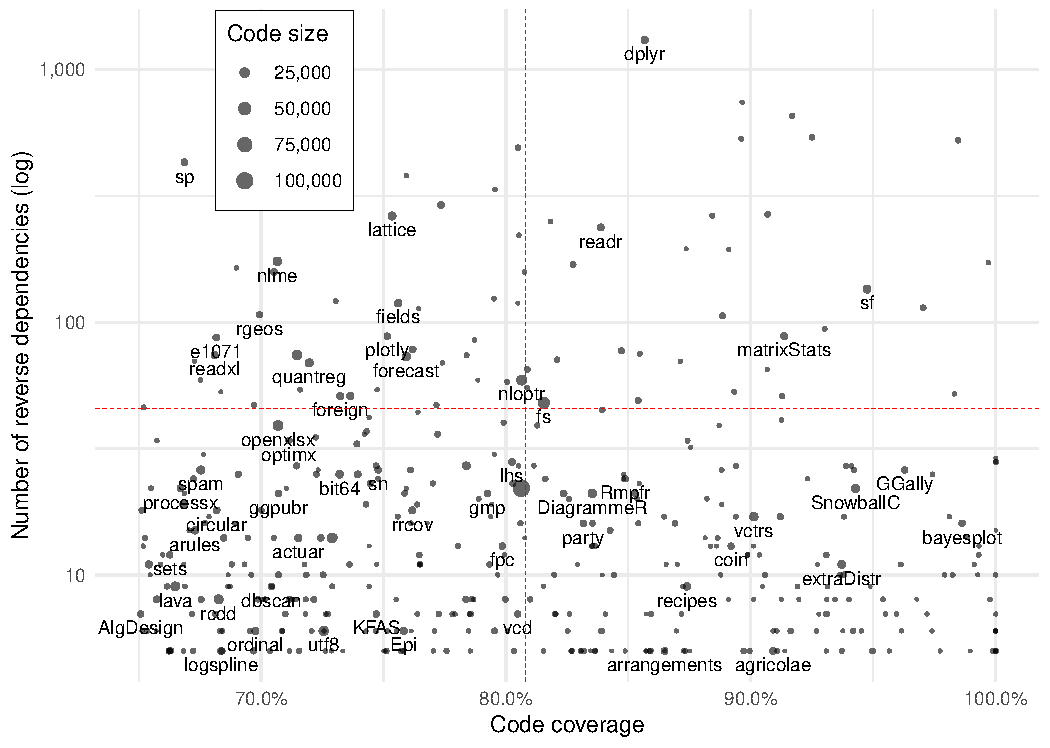
\includegraphics[width=.8\linewidth]{plots/corpus.pdf}
  \caption{Corpus overview}\label{fig:corpus}
\end{figure}

These packages come from the Comprehensive R Achive Network
(CRAN\footnote{\url{http://cran.r-project.org}}), the largest repository of
R code with over \AllCranRnd packages\footnote{CRAN receives about 6 new
  package submissions a day~\cite{Ligges2017}} containing over \AllRCodeRnd
and \AllNativeCodeRnd R and native code respectively. Unlike other open code
repositories like GitHub, CRAN is a curated repository. Each submitted
package must abide to a number of well-formedness rules that are
automatically checked asserting certain quality. Most relevant for this work
is that all of the runnable code (including code snippets from examples and
vignettes) is tested and only a successfully running package is admitted in
the archive.

We have downloaded and installed all available CRAN packages. Out of the
\AllCranRnd packages, we managed to install \AllLoadableRnd. The main reason
for this is that \rdt is based on R 3.5.0 and some of the packages are no
longer compatible with it. Some packages also require extra native
dependencies which were not present on our servers.  We have two criteria
for including a package into the corpus:
\begin{inparaenum}[(1)]
\item have runnable code that covers significant part of the package source
  code from which type signatures could be inferred, and
\item have some reverse dependencies that allows us to evaluate the inferred
types on runnable code from these dependent packages.
\end{inparaenum}
The concrete thresholds were set to at least \ThresholdCodeCoverage of
expression coverage and at minimum \ThresholdRevdeps reverse dependencies.

The code coverage was computed for each package using
\covr\footnote{\url{https://github.com/r-lib/covr}}, the R code coverage R
tool.  The reverse package dependencies were extracted from the package
metadata using builtin function.

%
%
%
%
%
%
\section{Methodology}

%
%
%
%
\subsection{typetracer and Initial Analysis}

To help inform the design of our type system, and to ensure that it aligns
with the day-to-day usage of R, we performed a corpus analysis of some of
the most widely used R packages.  The corpus is discussed in detail in
Section~\ref{sec:corpus}.  We built \typetracer, our dynamic analysis, in
the R-dyntrace~\cite{oopsla19} dynamic analysis framework which is itself
built on a modified version of R targeting R version 3.5.0---we refer the
reader to Section~\ref{sec:r-dyntrace} for more details on the framework.

%
%
\subsubsection{Overview}
The goal of our analysis is to discover argument types for functions,
builtins, and specials.  Naively intercepting function calls and recording
argument types is incorrect, as recall that R wraps arguments in promises
(Section \AT{what section}).  To circumvent this obstacle, we instead
intercept the forcing of promises: when a promise is forced, we identify the
surrounding call, collect the type of the value, and add it to the call
trace associated with the current function call.  Once function execution
completes, we collect information about the return value, add it to the call
trace, and save the completed call trace to be written out later.  \AT{This
  paragraph overlaps with the initial discussion of \contractr. We need to
  make sure that we don't inadvertently repeat ourselves.}

%
%
\subsubsection{Type Information}
Once a value is obtained, either on function return or when an argument
promise is forced, we probe the value for the following information:

\begin{itemize}
\item the value's type tag according to R's runtime. R's runtime implements
  type tags as a typedef, e.g. \code{INTSXP} for integers, and, confusingly,
  \code{VECSXP} for lists;
\item its class, which is a list of string class names. Typically, the class
  of a value is held in an attribute with name ``class'', though some
  classes are blessed by the R runtime, such as matrix and array classes;
\item its attributes, a list of metadata attached to the value.
\end{itemize}

Now, depending on the value's type tag, we collect further information:

\begin{itemize}
\item For R's primitive types, we collect its dimension, and if it has a
  names attribute we collect the names as well;
\item For lists, we recursively collect the types of list elements;
\item For lists {\it with a names attribute}, we collect the names as well as the types of the slots that those names refer to (data.frames fall into this category);
\item For promises, we carefully dig into the promise value {\it without
  forcing it}, and collect information about the innermost value. If the
  innermost value is the unbound value, then the promise is an as-of-yet
  unevaluated expression. In this case, we do our best to guess the value of
  the unevaluated expression: if the expression is not a language
  expression, we collect information about it, otherwise we can say nothing
  without evaluating it and ascribe it type ``any''. \footnote{\AT{I think
      this is confusing, reword.}}
\end{itemize}

For vectors (and lists), we additionally iterate through the elements,
checking if the values are NA (resp. NULL); if none are NA (resp. NULL), we
ascribe the NA-free (resp. NULL-free) tag to the value.  Arguments that are
part of a function's varargs (denoted \ldots in function definitions) are
tagged as such and ignored, as varargs can contain anything (and their type
will be equivalent to and any-typed list).

Now that we've seen the high-level picture of our approach, we will elaborate on some key details and discuss particular challenges that we faced.

%
%
\subsubsection{Challenges}
\label{subsec:typetracer-challenges}

We grappled with a number of corner cases related to R's non-strict semantics.

\begin{itemize}

\item First, we wanted to ensure that \typetracer captured type for
  unevaluated arguments.  Not every argument of a function needs to be used
  during every function execution, and the approach we discussed above
  relies on argument promises being forced (and, consequently, on arguments
  being used).  There are a few reasons for this.

One possibility is that the argument was simply unused given the control
flow of this particular execution (e.g. if the argument is only needed in
one branch of an \code{if}).  This mainly occurs when arguments have default
values for some parameters that are not critical to every execution oft he
function.  In these cases, we still want to collect the type of the default
value.

Another possibility is that a value is used {\it without being forced}, as
is the case when values are ``metaprogrammed'': \AT{describe, code example.}

To tackle this, we make an {\it initial guess} of function argument types on
function entry. This collects types for argument default values, and
collects an ``unused'' type for unevaluated expressions.  If an argument
promise is later forced, we simply update the recorded type for the
argument.

\item Second, we wanted to account for formal arguments (arguments which are
  named in the function definition) that were {\it not} passed to the
  function.  Put simply, a function was not called with all of its
  arguments, and no default value was specified for missing arguments.  In
  this case, we record a ``missing'' type for the argument.

There are two obvious ways to deal with missing arguments: type them as bot,
or as top.  As we are performing a dynamic analysis, based on package test
code, we conservatively type these arguments as top, or \code{any}.  It is
impossible to know dynamically what all possible function behaviours are,
\AT{I'm still not convinced about this.}

\item Third, we had to contend with R's C implementation sometimes
  performing longjumps, which discards current R calls from the call stack.
  In order to ensure that call traces are not lost when a longjump occurs,
  \typetracer intercepts the unwinding process initiated by the longjump and
  mimics the functionality of the functions being exited.  The R-dyntrace
  framework supplies the return value during the unwinding process (if there
  is indeed such a value), so we can capture it, analyze it, and include it
  in the call trace.  In certain situations, however, no return value can be
  obtained (e.g. a longjump occurred as part of some error handling), and
  then we simply record a ``jumped'' return value, which we can deal with in
  post-processing.  These longjumps occur quite often, particularly when S3
  dispatch occurs, as the R implementation optimizes returns from dispatched
  functions by initiating a longjump.

\end{itemize}

Having outlined these challenges, we will now explore the implementation of \typetracer in more detail.

%
%
\subsubsection{Select Details}

As mentioned, our analysis is built on the R-dyntrace framework.  R-dyntrace
is a very efficient instrumentation framework for R, which is built on a
modified version of the R runtime.  Our dynamic type analysis only needs to
be run once, ever---from the analysis results, we synthesize function
signatures which are passed along to later type-checking tools which do not
rely on a heavily modified runtime.

We primarily rely on 8 R-dyntrace callbacks: \texttt{closure\_entry},
\texttt{closure\_exit}, \texttt{builtin\_entry}, \texttt{builtin\_exit},
\texttt{special\_entry},\texttt{special\_exit},
\texttt{promise\_force\_entry}, and \texttt{promise\_force\_exit}.  These
callbacks fire when closures, builtin, and special functions are entered and
exited, and before and after the forcing of promises.  The function-related
callbacks are used mainly for bookkeeping: the analysis is notified that a
closure, builtin, or special has been entered/exited by pushing/popping the
call onto a stack.  The calls themselves store a {\it call trace} object,
where we store the type information that we collect, populated with initial
guesses of argument types (as discussed in
Section~\ref{subsec:typetracer-challenges}).  Further, the type of dispatch
is recorded on the {\tt \_entry} variants: \AT{recall} that there are
multiple ways that R performs dynamic dispatch, based on the class of
function arguments.  We collect dispatch information in order to analyze
dispatch usage patterns.

The main work is done in {\tt promise\_force\_exit}.  As arguments to
functions in R are wrapped in promises, we delay our reflection to promise
force time.  In R, promises are essentially objects with value and
expression slots.  When a promise is created for a particular expression,
that expression is merely put into the expression slot of a promise object,
and a special {\it unbound} value is loaded into the value slot (unless some
default value is specified, wherein it is loaded into the value slot---this
is the case with default argument values).  When the promise is forced, the
expression is evaluated in the forcing context, and the value is stored in
the value slot of the promise.  So to get the type of a function argument,
we check the value slot of the argument promise---perhaps recursively if the
value itself is a promise.

To construct a type for each argument, we make use of R's C FFI and use
low-level machinery to collect type tags and attributes from the R runtime.
The types that we provide to users are constructed during post-processing,
and rely on the detailed information made available by these low-level
reflection mechanisms.

%
%
%
%
\subsection{Post-Processing and Type Ascription}

The type information we collect is far more detailed than the types we
actually generate, and so the next stage of our inference process is to
distill the rich type information into simpler, manageable types.  For each
unique observed call trace, we translate the representation of the type of
each of the function arguments and returns according to the design of our
type system: for instance, we might have determined that a function returned
a vector of integer with 4 elements, with names, that was free of NA values,
in which case we would write out \code{integer[]} as the type.

Once types have been simplified in this way, for each function we move to
consolidate its multiple call traces into a single function type.  We do
this by combining the observed types of each argument into one type
(possibly a union, mind), according to subtyping rules that are part of our
design.  The precise subtyping rules we used will be discussed further in
Section~\ref{sec:typesystemdesign}.

While our analysis collects more detailed information than necessary for
type generation, the information proved useful for building up a usage
profile of the language. Through it, we were able to determine the best
translation rules (i.e., determining the type system we are translating to)
through an iterative process, involving analyzing usage patterns that arose
in the data and making design decisions based on them, revisiting the data
as necessary.  In the following section, we will discuss these decisions in
more detail, highlighting the reasoning behind our type system design.

%
%
%
%
%
%
\section{Type Language Design}
\label{sec:typesystemdesign}

Our corpora analysis reported \AT{number} call traces for over \AT{number}
functions.  We distilled these call traces into function types which
captured the dynamic behaviour of the functions.  We emphasize that this was
an iterative process: initial analysis suggested a certain set of types,
which we tried and implemented, and reanalysis suggested improvements,
and so on.  In this section, we will present the final type annotation language design, 
which we believe captures the essence of R.  Throughout, we will
touch on design decisions and weigh our choices against alternatives,
speaking to the strengths and weaknesses of our chosen design.
We begin with basic, primitive types.

%
%
%
%
\subsection{Basic Types}
\label{subsec:basictypes}

As discussed in Section~\ref{subsubsec:backgroundtypes}, the workhorse types
in R are the vectorized primitives: integers, doubles, complex numbers,
logicals (booleans), characters, and raws (bytes).  These are {\it
  vectorized} in that they are always considered to be vectors by the R
runtime: for instance, even ``scalar'' numbers are considered to be
unit-length vectors to R.  These primitive vectors are homogeneous, in that
a vector of doubles contains only doubles.

Related to these primitive types is one of R's notions of ``nullness'': for
each of the primitives, R distinguishes a special ``NA'' value which
represents missing data.  There is an NA for each of the primitive types
(i.e. there is a double NA, integer NA, etc.).  Thus, even homogeneous
vectors can represent missing data with their appropriate NA value.

As with everything in R, there is nuance in even the simplest cases.
We will now discuss our design decisions relating to the vectorized primitives.

%
%
\subsubsection{Possibly-NA Primitives}

A common primitive usage pattern is related to the presence of NAs:
\AT{often}, programmers explicitly check for NAs in primitive vectors,
possibly sanitizing them if they are present.  NAs complicate practically every computation
using primitive vectors, a fact that many programmers appear to be acutely
aware of. For instance, consider the code in Figure~\ref{fig:na-example}.

\begin{figure}[htbp]
\begin{center}

\begin{lstlisting}
binom.profile <- function(x, n, ...) {
  xn <- cbind(x = x, n = n)
  ok <- !is.na(xn[, 1]) & !is.na(xn[, 2])
  x <- xn[ok, "x"]
  n <- xn[ok, "n"]
  ...
\end{lstlisting}

\caption{NA checking example from the \code{binom} package.}
\label{fig:na-example}
\end{center}
\end{figure}

The \code{binom} package is a popular package \AT{do we want e.g. \# revdeps?} for computing confidence intervals for binomial experiments, and the \code{binom.profile} function does so using the profile likelihood, the details of which are not relevant here.
Here, we highlighted a relevant snippet of code, which appears at the beginning of the function: the programmer first binds the vectors into a matrix (line 2), with one column for each of \code{x} and \code{n}, then finds rows where both columns are not NA (line 3), then extracts non-NA values and stores them into \code{x} and \code{n} respectively (lines 4-5).
Importantly, this process is entirely quiet, and the user of \code{binom.profile} will not be notified if their data happens to contain NAs, and the NAs will be silently ignored. 
In reality, the presence of NAs in data could signify some sort of data corruption, and quietly ignoring issues in data could lead users (read: statisticians) to draw flawed conclusions from erroneous data.

To combat this, we introduce a modifier on primitive types: the type \code{^T} signifies that primitive type \code{T} might contain an NA value, while \code{T} signifies that \code{T} is NA-free. 
If the \code{binom} developers were to annotate arguments \code{x} and \code{n} with such an NA-free type, \contractr will notify users when \code{binom.profile} is called with NA-full values, rather than just quietly ignoring them.
\AT{Gather usage statistics.}

Note that when combining call traces involving \code{^T} and \code{T} types, we subsume \code{T} types into \code{^T} types: if NA-free and NA-full vectors are passed to an argument, then we say that the argument can handle NA-full vectors.
This is equivalent to \code{T <: ^T}. 

%
%
\subsubsection{Scalar Primitives}

Initial analyses of our data revealed that programmers \AT{often} use scalars (as explicitly as they can, anyway), and often do high-level dimensionality checks on their data.
To illustrate, consider the code in Figure~\ref{fig:scalar-vector-example}.

\begin{figure}[htbp]
\begin{center}

\begin{lstlisting}
hankel.matrix <- function( n, x ) { 
### arguments
### n = a positive integer value for the order of the Hankel matrix
### x = an order 2 * n + 1 vector of numeric values
    ...
    if ( n != trunc( n ) )
        stop( "argument n ix not an integer" )
    if ( !is.vector( x ) )
        stop( "argument x is not a vector" )
    m <- length( x )
    if ( m < n )
        stop( "length of argument x is less than n" )
    ...
\end{lstlisting}

\caption{Scalar/vector example from the \code{matrixcalc} package.}
\label{fig:scalar-vector-example}
\end{center}
\end{figure}

The \code{hankel.matrix} function takes two arguments (as described in the comment in the code), and returns a Hankel matrix, which essentially is a matrix where the skew-diagonals have a desirable property.
The function body has a number of interesting checks:
on lines 6-7, \code{n} undergoes an integer ``type check'';
on lines 8-9, \code{x} undergoes a vector ``type check'';
on lines 11-12, \code{n} is assumed to be a scalar (if it were a vector, R would generate a warning, as \code{m < n} would return a vector of logicals obtained from checking if \code{m} were less than each element of \code{n} \AT{do we want to put the warning here?}).
These checks exemplify behaviour we would like to capture with our annotation language, as we would like to differentiate between scalars and vectors in addition to checking for the basic type of a value (e.g. integer vs double), 

To that end, we introduce the following types into our type language:
for some primitive type \code{T}, the user may modify \code{T} with a modifier \code{[]} to indicate that it is a vector of \code{T}.
Perhaps surprisingly, we found that scalars occurred more often than vectors, and chose the scalar type syntax as the default. 
The NA-free modifier works as expected: \code{^T[]} indicates a vector of \code{T} that is free of NAs, while \code{^T} indicates a scalar which is not NA.
 
%
%
\subsubsection{Matrices}

On the subject of matrices, they represent another layer of complexity on top of vectorized primitives.
Internally, matrices are simply vectors with class ``matrix'' and a \code{dims} attribute indicating matrix dimensions, and many functions automatically coerce vectors to matrices when appropriate (while not codified in the language semantics, many internal functions perform the coercion).
Relying on automatic coercion is unwise, and many functions check to ensure that their arguments are matrices, particularly those in packages which rely on matrices.
For instance, consider the code in Figure~\ref{fig:matrix-example}.

\begin{figure}[htbp]
\begin{center}

\begin{lstlisting}
rowWeightedMeans <- function(x, w = NULL, rows = NULL, cols = NULL,
                             na.rm = FALSE, ...) {
  # - - - - - - - - - - - - - - - - - - - - - - - - - - - - - - - - - - - - -
  # Validate arguments
  # - - - - - - - - - - - - - - - - - - - - - - - - - - - - - - - - - - - - -
  # Argument 'x':
  if (!is.matrix(x)) {
    .Defunct(msg = sprintf("Argument 'x' is of class %s, but should be a matrix. 
    The use of a %s is not supported, the correctness of the result is not guaranteed. 
    Please update your code accordingly.", sQuote(class(x)[1]), sQuote(class(x)[1])))
  }
  ...
\end{lstlisting}

\caption{Matrix example from the \code{matrixStats} package.}
\label{fig:matrix-example}
\end{center}
\end{figure}

The \code{rowWeightedMeans} function calculated the weighted means of rows or columns of a matrix \code{x}.
This function exhibits good practice in type checking arguments, rightly producing a message to the user indicating that an explicit matrix should be passed.

To capture cases like this, we include a \code{class<matrix>} type in our type annotation language.
If \code{rowWeightedMeans} were outfitted with such a type, \contractr can perform the check present in this code automatically.
That said, we don't' intend to subsume all validation code, a topic we discuss next.
 
%
%
\subsubsection{Forgoing Dimensionality} 



\AT{Will revisit to tighten discussion, need to think about best way to
  phrase this.  Perhaps "dependent type system bad" is enough?}  Including
data dimensions in types would make our type system a dependent type system,
which we believe is too complex to retrofit onto a dynamic data science
language such as R.  The simplest way to include dimensions would be to
explicitly specify the dimensions of an argument (e.g. specifying that a
function should always be called with a double vector of length 10), which
is not particularly useful, and a pattern which \AT{rarely appeared in our
  analysis}.



%
%
%
%
\subsection{Lists}

\AT{List rehash.}  Separate from the vectorized primitives in R are lists:
Whereas vectors are homogeneous and restricted to primitive types, lists can
contain arbitrarily-typed data.  R even builds on lists to create a more
complex data structure known as the {\it data frame}, an essential data
structure to R's functionality \AT{maybe too aggressively worded, but we can
  back this up with data, e.g. how many functions take data frames?}.

\AT{Outline concerns for typing.}  We are faced with several possible
designs for list types.  Chief concerns include the heterogeneity of list
elements, and the presence of a \code{names} attribute, allowing list
elements to be accessed in a struct-like manner.  \AT{Rarely?}, programmers
even write code expecting lists of a particular pre-defined length.  The
next sections highlight some important design decisions for our list types.

\AT{Dig into concerns for typing.}

%
%
\subsubsection{Forgoing Tuples, or Short, Constant Length Lists}

We briefly entertained the possibility of including a \code{tuple} type,
which would have looked like e.g. \code{tuple<int, int>} for a list of two
integers.  When configured to detect tuples, our analysis did indeed pick up
\AT{a number}, but post-processing and simplification revealed that in
\AT{many} cases, they would be subsumed by co-occurring \code{list} types.
In other words, it just so happened that functions were being called with
short lists.  Of the cases that tuples were not subsumed by lists,
\AT{often} there were \AT{tuples of different lengths}, implying that the
shape of the argument was not essential.  \AT{Wording...}

%
%
\subsubsection{Forgoing Structs}

Another pattern that we observed was the use of consistently-named lists.
In R, ``fields'' of named lists can be accessed using the \code{$} operator,
such as:
\begin{lstlisting}
p <- list(x=1, y=2)
p$x + p$y
\end{lstlisting}
We thought to capture this type of behaviour with a {\it struct} type, such
as \code{struct<x: integer, y: integer>}.  Initial analyses suggested that
structs were very common, but further inspection revealed that they failed
to tell the full story.  For instance, \AT{many} structs were merely
representing list-typed values with a {\it class}, and we could capture
these types more succinctly with a class-based type.  Further, it is common
in R example code to use some built-in data sets, such as \AT{mention some}.
These caused undue noise, as even with our struct name unification strategy,
poorly tested functions appeared to operate on e.g. \AT{funny struct type
  from the previous data set}.  Ultimately, we found that sticking to list
types and adding a class-based was the wisest course of action.  We will
discuss class types shortly.

%
%
\subsubsection{Forgoing Data Frames}

Speaking of classes, an important classful value in R is the data frame.
Data frames underpin nearly all idiomatic use of the language, and even
popular \code{tibble} (from the \code{tidyverse} ecosystem) and
\code{data.table} (from the \code{data.table} package) build on the
essential type.  We entertained the possibility of including data frame
types, but \AT{found them to be clunky? Question mark?}  Consider:
\AT{example of why data.frame types would be bad atm.}

Data frames do have a type, through the \code{class<data.frame>} type, and
future work will expand on this type, discussed further in
Section~\ref{sec:futurework}.

%
%
%
%
\subsection{Classes in R}

As discussed in Section~\ref{sec:R}, the R runtime has more than one notion
of type.  The {\it class} (rather, the {\it classes}, as values can have
multiple!) of function arguments are used by R to {\it dispatch} the correct
function call for the argument \AT{$\leftarrow$ wording}.  This is best
served with an example: \AT{Example, unless we talked about this earlier, in
  which case refer reader back.}

%
%
\subsubsection{Class Types}

The class of a value suggest a shape for the value, and we felt class to be a more succinct way of capturing struct-like types. 

\AT{We used classes to stand-in for structs.  The discussion here is
  naturally tied with the discussion of structs, so we need to make sure to
  divide the discussion appropriately.}

%
%
\subsubsection{Multi-Classes}

As R does, our type system supports multiple classes on values, and the type
of a classful value is simply a list of all of its classes.

\AT{What more to say here? Discussing occurrences of multi-classes?}

%
%
\subsubsection{Forgoing R's Object Systems}

R has multiple, disparate object systems, with the language providing direct
support for S3, S4, and R5.  Thus far, we've mainly discussed S3 and its
dispatch mechanism, and indeed our class types roughly capture the S3
``types'' of values.  We will not discuss R5 as it is still under
development.

For S4, we have an \code{s4} type to denote S4 values, though we did not
elaborate on this type.  We stuck to simple S4 types since doing anything
more would be immensely complicated, and outside of the scope of this work.
For instance, the mechanics of S4 dispatch are more complex than for S3 (S4
dispatches on the class of {\it all} arguments), and users can define their
own class hierarchies that we would need to incorporate in our type analysis
and contract checking frameworks.  Further, \AT{we found limited use of S4
  during our analysis}, with S4 types being heavily used in a select subset
of packages (\AT{such as ...}), some of which make heavy use of R's
metaprogramming capabilities.  Coming up with a type system that accounts
for all of these factors, and consolidates multiple object-orientation
frameworks, is an interesting problem in and of itself, and we aim to extend
our type system to account for this in future work.  For now, S3 types
suffice: S3 is the most common object system in R, with no sophisticated
hierarchies, and its semantics are simple enough to be captured by our
proposed design.

%
%
%
%
\subsection{Final Type Grammar}
\label{subsec:typegrammar}

\begin{figure}          % Types
    \noindent           % Collapse for readability.
    \centering
    \begin{minipage}{.45\linewidth}
    \begin{flushleft}
    % Types
      $ \begin{array}{lclr}
    D & ::= & {\bf type} \; ID \; T {\bf ;}  & \text{\it type declaration}\\
    T & ::= & {\bf null} & \text{\it unit type} \\
      & |   & {\bf any} & \text{\it top type} \\
      & |   & {\bf environment} & \text{\it environment type} \\
      & |   & {\bf expression} & \text{\it expression type} \\
      & |   & {\bf language} & \text{\it language type} \\
      & |   & {\bf symbol} & \text{\it symbol type} \\
      & |   & {\bf externalptr} & \text{\it externalptr type} \\
      & |   & {\bf pairlist} & \text{\it pairlist type} \\
      & |   & {\bf s4} & \text{\it S4 type} \\
      & |   & {\bf weakref} & \text{\it weakref type} \\
      & |   & S & \text{\it scalar type} \\
      & |   & V & \text{\it vector type} \\
      & |   & \left( T \right) & \text{\it group type} \\
      & |   & T_1 \; {\bf |} \; T_2 & \text{\it union type} \\
      & |   & \langle A_1 , ..., A_n\rangle \Rightarrow T & \text{\it function type} \\
      & |   & {\bf struct}\langle F_1, ..., F_n \rangle & \text{\it struct type} \\
      & |   & {\bf list} \langle T \rangle & \text{\it list type}\\
      & |   & {\bf class}\langle ID_1, ..., ID_n \rangle & \text{\it class type}\vspace{5pt}\\
    \end{array} $
    \end{flushleft}
    \end{minipage}
    \hfill
    \begin{minipage}{.45\linewidth}
    \begin{flushright}
    $ \begin{array}{lclr}
    % Argument Types
    A & ::= & T & \text{\it argument type} \\
      & |   & {\bf ...} \vspace{5pt} \\
    % Field Types
    F & ::= & ID : T & \text{\it struct field}\vspace{5pt}\\
    % Scalar Types
    S & ::= & B & \text{\it scalar types} \\
      & |   & N \vspace{5pt}\\
    % Vector Types
    V & ::= & S \lbrack \rbrack & \text{\it vector types} \vspace{5pt}\\
    % Base Types
    B & ::= & {\bf int} & \text{\it base types} \\
      & |   & {\bf chr} \\
      & |   & {\bf dbl} \\
      & |   & {\bf lgl} \\
      & |   & {\bf clx} \\
      & |   & {\bf raw} \vspace{5pt}\\
    % NA Types
    N & ::= & {\bf \string^int} & \text{\it na types} \\
      & |   & {\bf \string^chr} \\
      & |   & {\bf \string^dbl} \\
      & |   & {\bf \string^lgl} \\
      & |   & {\bf \string^clx} \\
\end{array} $
    \end{flushright}
    \end{minipage}
    \caption{The R type system.}
    \label{fig:types}
\end{figure}

%
%
%
%
%
%
\section{Evaluation Results}
\label{sec:evaluation}

We contended with multiple type language designs, and in this section we will explore in more detail how we compared our candidate designs.
We will also discuss a large-scale evaluation of our final set of type annotations.

%
%
%
%
\subsection{Comparative Analyses}

\AT{We compared different designs: with/out structs and tuples, with/out classes, with/out primitive subtyping. We looked at type sizes and determined that e.g. \code{? T} is a good type.}

%
%
\subsubsection{Analysis of Polymorphism}

\AT{How many arguments, functions are polymorphic? How many packages? Are there pathologically polymorphic packages? Why didn't you handle those?}

%
%
\subsubsection{Use of \code{any}}

\AT{When is any introduced? Why? How does it affect the results? What if missing/unused isn't any, do the results change substantially?}

%
%
%
%
\subsection{Large-Scale Evaluation}

Now that we have settled on a language design, we endeavour to evaluate it against a representative subset of existing R code.
To this end, we took the detailed type information we collected from \AT{corpus} popular R packages, inferred types for the functions exposed by those packages, and ran the test, example, and vignette code of each of their reverse dependencies.

%
%
\subsubsection{Experiment Setup}

\AT{What is the design of the experiment? The setup? How much code was ran? What does this evaluate? Why does it mean anything for the annotation framework?}

\typetracer is capable of inferring type signatures based on the call traces it has collected.
These call traces were consolidated into a single function type for each package function:
\typetracer employs unification strategies discussed in Section~\ref{sec:typesystemdesign} to keep the size of signatures in check and only generates an \code{any} type under extenuating circumstances: when inner list types got too big (we decided to cap the union type in lists to 5), when missing and unused arguments were recored, and finally when a longjump caused function execution to abort prematurely.
Finally, we loaded each of these inferred types into \contractr, and ran all example code from the reverse dependencies of these popular packages.

%
%
\subsubsection{Results}

\AT{How many failing assertions? How many functions had these failed assertions? Which packages? How was the coverage? What are patterns in the actual types of the failed assertions? In the expected types? How many times did the code trigger the contracts?}

Overall, we found that only \AT{2\%} of contract assertions failed.
\AT{What does this indicate? One thought:}
This indicates two things: firstly, the corpus of packages we selected is quite well-tested, and much of the intended function behaviour is exemplified in the package example code. 
Secondly, and more importantly, this success indicates that our analysis framework is able to generate function types which accurately capture the behaviour of the function. 
\AT{It kind of feels like these need to simultaneously be true. Maybe we pull in the fact that coverage is good?}

Of the \AT{2\%} of failing contract assertions, we picked up on a few significant patterns.
Firstly, we found that \AT{10\%} of the failing assertions were due to \code{double}-typed values being passed to function arguments expecting an \code{integer}.
While we cannot say for sure that {\it all} of these cases could be handled by coercion, it is worth noting that coercion from doubles to integers is exceedingly common in R: the practice is not codified in the language spec, but many of R's internal C functions explicitly perform this coercion.
\AT{We can put an example, e.g. nrow(df) is an integer but 5 is not. Also list access coerces the double to an int.}

Next, \AT{30\%} of failing assertions were due to vector-typed primitive values being passed to function arguments expecting a \code{class<matrix>}.
This case exemplifies something we have touched on earlier, namely that vectors can be readily considered to be unidimensional matrices.
\AT{Is this coercion automatic? I've seen it mentioned often in the documentation.}

Separately, we investigated the effect of running reverse dependency code on the code coverage of the packages in our corpus.
We found that \AT{in many cases}. the reverse dependencies increased the code coverage (this aligns with findings in \AT{cite genthat}), and this was especially true for the functions for which contract assertions failed.

%
%
%
%
%
%
\section{Related Work}
\label{sec:relatedwork}

\AT{Good to mention the related projects, e.g. how this was undertaken in
  other languages, like Ruby.  There's a lot of literature in that space I
  think, I've read some of it but not all.  We also have some related work
  in the old paper, I'll grab it and put it here.}

%
%
%
%
%
%
\section{Conclusion}

\ldots

%
%
%
%
\subsection{Threats to Validity}

\subsection{Future Work}

\bibliography{bib/biblio,bib/jv,bib/r,bib/new,bib/gradual}

\end{document}
\appendix
\section{Appendix}
